\section{Kiến trúc phát triển (Development View)}
\begin{figure}[H]
	\centering
	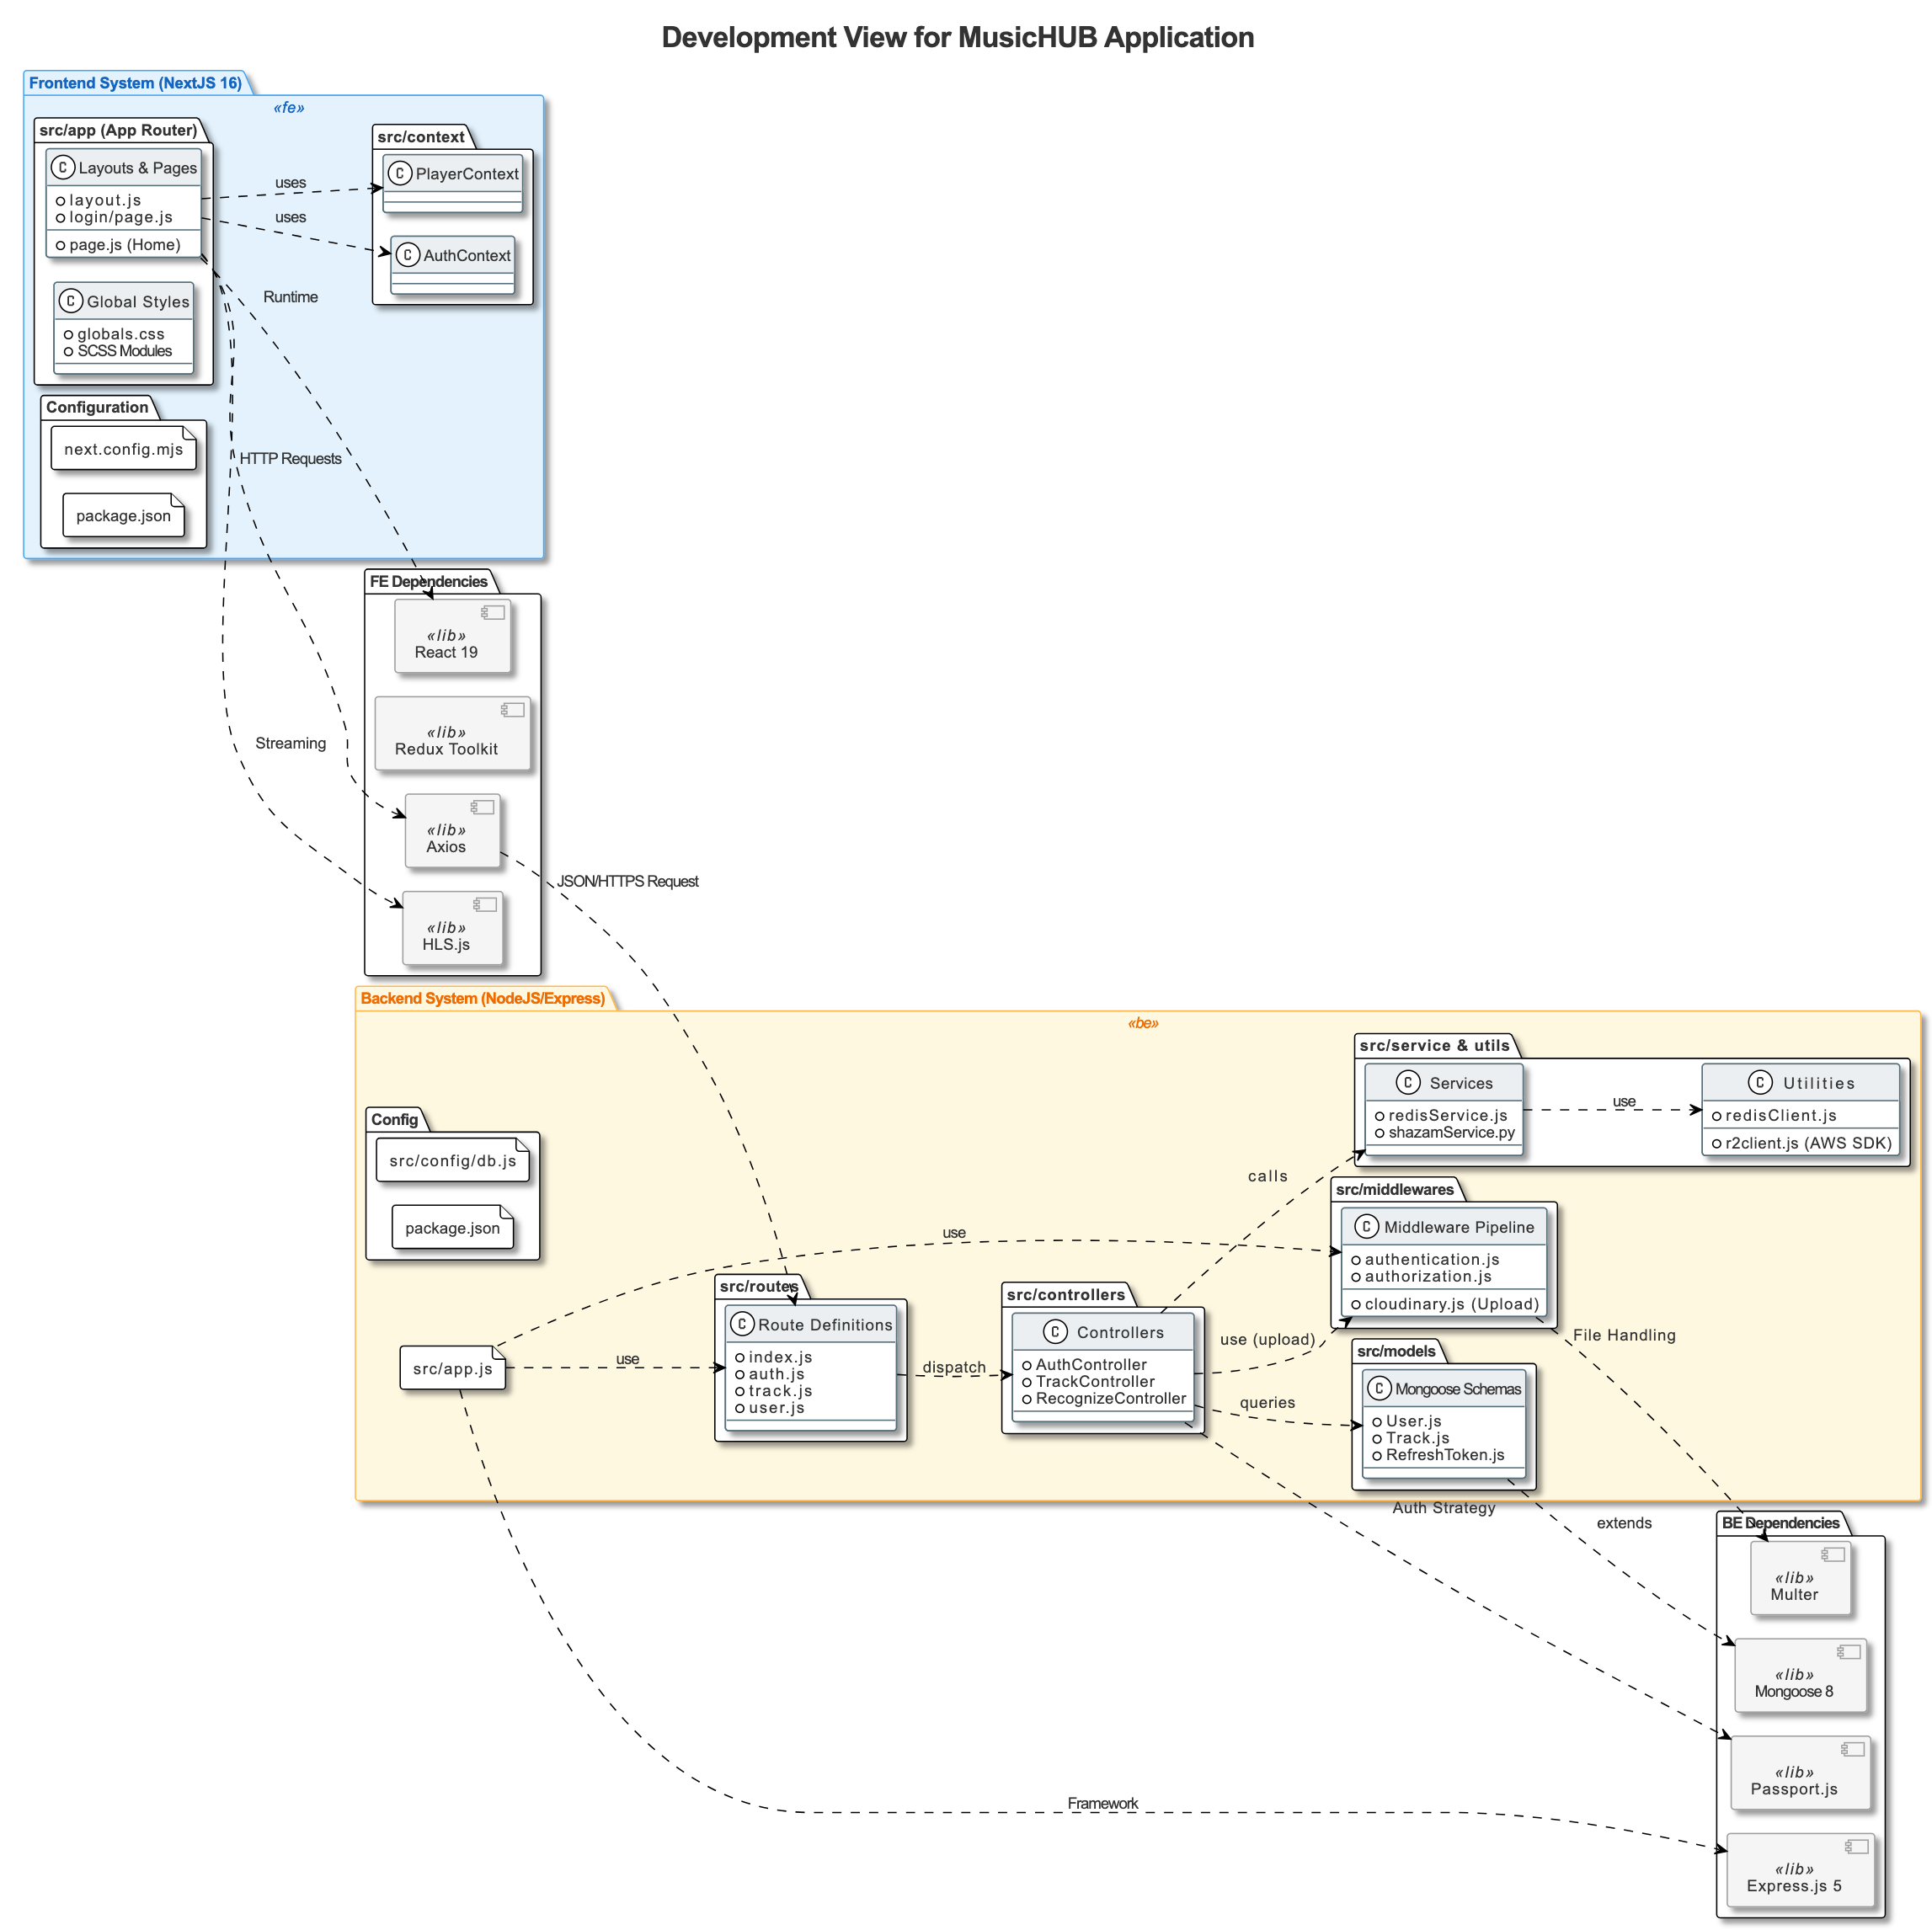
\includegraphics[width=\textwidth]{Images/development.png}
	\caption{Development View của hệ thống}
\end{figure}

\subsection{Tổng quan}
Development View mô tả cách tổ chức mã nguồn, cấu trúc module và quản lý sự phụ thuộc (Dependencies) của hệ thống MusicHUB. Hệ thống được phát triển theo mô hình tách biệt hoàn toàn (Decoupled Architecture) giữa Frontend và Backend, cho phép hai phía được phát triển độc lập.

\subsection{Tổ chức mã nguồn (Source Code Organization)}

Hệ thống được chia thành hai thư mục gốc (monorepo-style structure):
\begin{itemize}
    \item \textbf{\texttt{fe/}}: Chứa toàn bộ mã nguồn Frontend (Next.js).
    \item \textbf{\texttt{be/}}: Chứa toàn bộ mã nguồn Backend (Node.js).
\end{itemize}

\subsubsection{Phân hệ Frontend (\texttt{fe/})}
Được xây dựng dựa trên \textbf{Next.js 16} và \textbf{React 19}, cấu trúc mã nguồn tuân theo kiến trúc \textit{App Router} hiện đại:

\begin{itemize}
    \item \textbf{\texttt{src/app/}}: Chứa các trang (Pages) và Layout. Đây là tầng giao diện (Presentation Layer), nơi định nghĩa các đường dẫn (Routes) và cấu trúc UI.
    \item \textbf{\texttt{src/context/}}: Quản lý trạng thái toàn cục (Global State) sử dụng React Context API.
    \begin{itemize}
        \item \texttt{AuthContext.js}: Quản lý phiên đăng nhập, token người dùng.
        \item \texttt{PlayerContext.js}: Quản lý trình phát nhạc (Play, Pause, Seek, Playlist queue).
    \end{itemize}
    \item \textbf{\texttt{Dependencies}}:
    \begin{itemize}
        \item Giao diện: SCSS Modules, FontAwesome, React Icons.
        \item Xử lý Media: \texttt{hls.js} (Streaming audio), \texttt{react-virtuoso} (Danh sách ảo hóa hiệu năng cao).
        \item Giao tiếp: \texttt{Axios} (HTTP Client).
    \end{itemize}
\end{itemize}

\subsubsection{Phân hệ Backend (\texttt{be/})}
Được xây dựng dựa trên \textbf{Express.js 5}, tổ chức theo mô hình \textbf{MVC (Model-View-Controller)} kết hợp với kiến trúc phân lớp (Layered Architecture):

\begin{itemize}
    \item \textbf{\texttt{src/app.js}}: Điểm khởi chạy (Entry Point), nạp các cấu hình và middleware toàn cục.
    \item \textbf{\texttt{src/routes/}}: Định nghĩa các API Endpoint và điều hướng request đến Controller tương ứng.
    \item \textbf{\texttt{src/controllers/}}: Tầng xử lý nghiệp vụ (Business Logic).
    \begin{itemize}
        \item \texttt{AuthController}: Xử lý logic đăng nhập (Local \& OAuth).
        \item \texttt{TrackController}: Xử lý logic upload và streaming nhạc.
        \item \texttt{RecognizeController}: Điều phối tiến trình nhận diện nhạc.
    \end{itemize}
    \item \textbf{\texttt{src/models/}}: Tầng truy cập dữ liệu (Data Access Layer), định nghĩa các Schema Mongoose (\texttt{User}, \texttt{Track}, \texttt{Playlist}).
    \item \textbf{\texttt{src/middlewares/}}: Các bộ lọc xử lý request pipeline (Authentication, Authorization, File Upload qua Cloudinary).
    \item \textbf{\texttt{src/service/}}: Các dịch vụ tích hợp đặc thù.
    \begin{itemize}
        \item \texttt{shazamService.py}: Script Python tích hợp để xử lý tín hiệu âm thanh.
        \item \texttt{redisService.js}: Service tương tác với Redis Cache.
    \end{itemize}
\end{itemize}

\subsection{Công nghệ sử dụng (Technology Stack)}

\begin{table}[H]
\centering
\begin{tabular}{|l|l|l|}
\hline
\textbf{Phân hệ} & \textbf{Hạng mục} & \textbf{Công nghệ / Thư viện} \\ \hline
\multirow{4}{*}{Frontend} & Core Framework & Next.js 16, React 19 \\ \cline{2-3} 
 & State Management & React Context, Redux Toolkit \\ \cline{2-3} 
 & Media & HLS.js \\ \cline{2-3} 
 & Styling & SCSS, CSS Modules \\ \hline
\multirow{4}{*}{Backend} & Runtime & Node.js, Express.js 5 \\ \cline{2-3} 
 & Database & Mongoose (MongoDB ODM), IORedis \\ \cline{2-3} 
 & Authentication & Passport.js, JWT, Bcrypt \\ \cline{2-3} 
 & File Processing & Multer, Cloudinary SDK, AWS S3 SDK \\ \hline
\end{tabular}
\caption{Danh sách các công nghệ và thư viện chính}
\end{table}

\subsection{Quy trình phát triển (Development Workflow)}
\begin{enumerate}
    \item \textbf{Môi trường:} Sử dụng biến môi trường (\texttt{.env}) để quản lý cấu hình nhạy cảm (DB Connection, API Keys) riêng biệt cho Development và Production.
    \item \textbf{Frontend Dev:} Chạy trên port 3000 với tính năng Hot Module Replacement (HMR) của Next.js.
    \item \textbf{Backend Dev:} Chạy trên port 8080 sử dụng \texttt{nodemon} để tự động khởi động lại server khi thay đổi code.
    \item \textbf{Inter-communication:} Frontend giao tiếp với Backend thông qua RESTful API, sử dụng JWT Bearer Token trong Header để xác thực.
\end{enumerate}